\documentclass{amsart}

\usepackage[notref,notcite]{showkeys}
\usepackage[style=authoryear,ibidtracker=false,uniquename=false,giveninits=true,terseinits=true,maxbibnames=5,backend=biber]{biblatex}
\usepackage{float}
\usepackage{graphicx}

\renewbibmacro{in:}{}
\addbibresource{rnni_polynomial.bib}

\newtheorem{lemma}{Lemma}

\newcommand{\rnni}{\mathrm{RNNI}}
\newcommand{\findpath}{\textsc{FindPath}}
\newcommand{\mrca}{\mathrm{mrca}}
\newcommand{\rank}{\mathrm{rank}}
\newcommand{\nni}{\mathrm{NNI}}

\graphicspath{{figures/}}

\begin{document}

\begin{lemma}
Let $T$ and $R$ be $\rnni$ trees such that $\findpath(T, R)$ terminates after two iterations and returns a path $p$ of length $\ell$.
Then $\ell = d(T, R)$.
\end{lemma}

\proof
Case 1: $R = [\{1, 2\}, \{3, 4\}, \ldots]$.

Let $T'$ be the running tree after the first iteration of $\findpath(T, R)$.
Define
\[
s(T, R) = (\rank(\{1,2\})_T - 1) + (\rank(\{3,4\})_{T'} - 2)
\]
where $\rank(S)_T$ is the rank of the most recent common ancestor of cluster $S$ in tree $T$.
Note that an inductive argument implies that it is enough to show that $s(T_1, R) \geq s(T, R) - 1$ for all $T_1 \in N_1(T)$.
This means that there is no tree $T_1 \in N_1(T)$ that is more than one $\rnni$ move closer to $R$ than $T$.

For the following it is important to notice that the following holds for the path $p$ computed by $\findpath(T,R)$.
If $\mrca_T(\{1,2\}) > \mrca_T(\{3,4\})$, then there is no tree on $p$ where $\mrca(\{1,2\}) = \mrca(\{3,4\})$.

If this was possible on $p$, it could only result from an $\nni$ move that moves $\mrca(\{1,2\})$ down, and not from a rank swap.
An $\nni$ move that moves $\mrca(\{1,2\})$ down exchanges two subtrees, one of them containing taxon $1$ or $2$, the other one none of the two.
Let us call these are the subtrees $B$ and $C$ of Figure~\ref{fig:nni_move}, and without loss of generality assume that $1 \in A$ and $2 \in B$.
If after this move it is $\mrca(\{1,2\}) = \mrca(\{3,4\})$, then one of the taxa $3,4$ is in $A$ and the other one in $C$.
But then it must have been $\mrca(\{1,2\}) = \mrca(\{3,4\})$ in the tree just before this $\nni$ move already.
Therefore, it cannot be $\mrca(\{1,2\}) = \mrca(\{3,4\})$ on a tree on $p$, if it is $\mrca_T(\{1,2\}) \neq \mrca_T(\{3,4\})$ in the start tree $T$.


\begin{figure}[H]
\centering
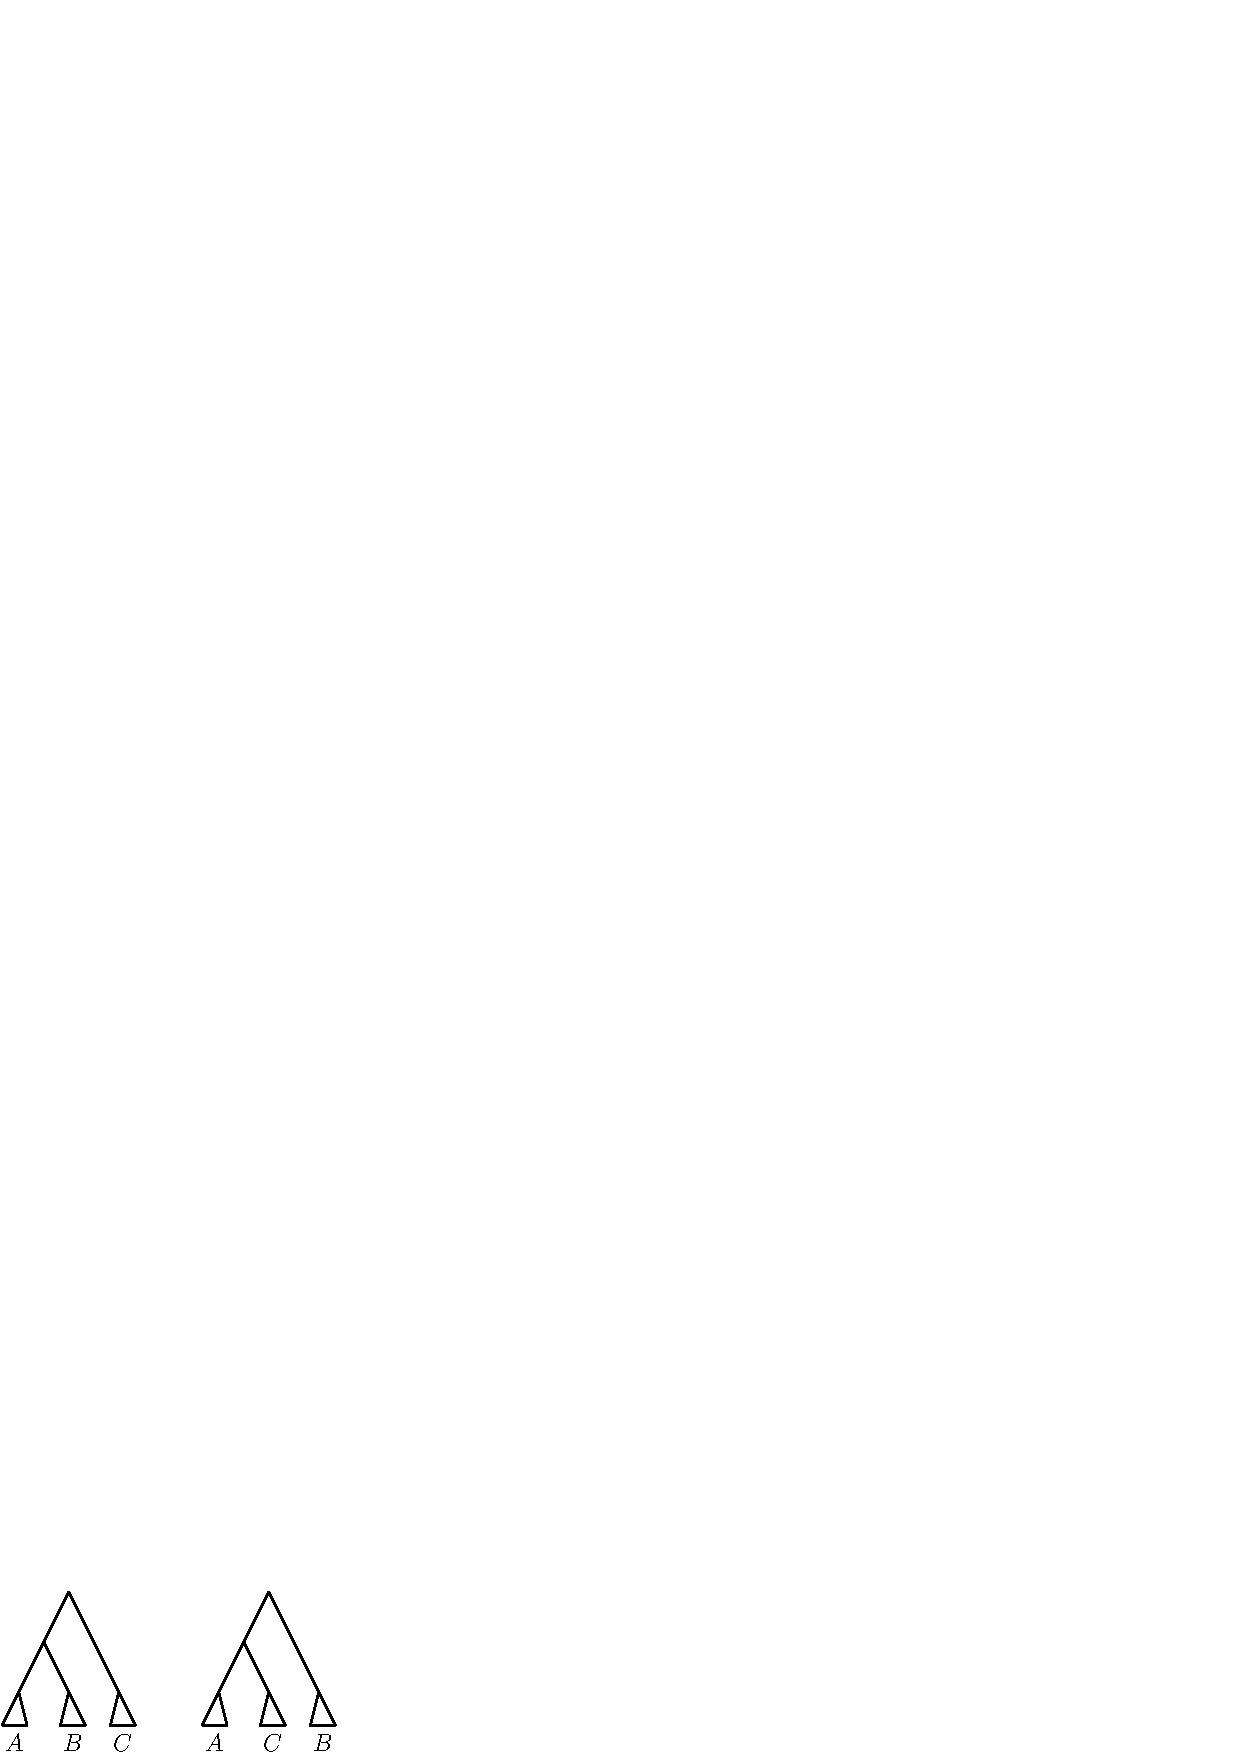
\includegraphics[width=0.4\textwidth]{NNI_move}
\vspace{12pt}
\caption{$\nni$ move}
\label{fig:nni_move}
\end{figure}

So let now $T_1 \in N_1(T)$ and let $T''$ be the tree after the first iteration of $\findpath(T_1,R)$. We will distinguish different possible $\rnni$ moves between $T$ and $T_1$ and consider how the path $\findpath(T_1,R)$ changes compared to $\findpath(T,R)$.

\begin{enumerate}

    \item The $\rnni$ move between $T$ and $T_1$ does not change the rank of $\mrca(\{1,2\})$ or $\mrca(\{3,4\})$

    It is obvious that $\rank(\{1,2\})_{T_1} = \rank(\{1,2\})_{T}$ as well as $\rank(\{3,4\})_{T''} = \rank(\{3,4\})_{T'}$, as the move between $T$ and $T_1$ does not have an effect of the ranks of these most recent common ancestors in $T$ or $T'$.
    Therefore, it is $s(T, R) = s(T_1,R)$.

    \item The $\rnni$ move between $T$ and $T_1$ changes $\rank(\mrca(\{1,2\}))$, which is not equal to $\rank(\mrca(\{3,4\}))$

    If this $\rnni$ move increases the rank of $\mrca(\{1,2\})$, the first move on $\findpath(T_1,R)$ will decrease the rank of this most recent common ancestor and results in the tree $T$, which gives us $\rank(\{1,2\})_{T_1} = \rank(\{1,2\})_{T} - 1$.
    If otherwise the rank of $\mrca(\{1,2\})$ decreases by the $\rnni$ move from $T$ to $T_1$, it is $\rank(\{1,2\})_{T_1} = \rank(\{1,2\})_T - 1$.
    However, the rank of $\mrca(\{3,4\})$ is the same in $T'$ and $T''$, no matter whether $\rank(\mrca(\{1,2\}))$ decreases or increases.
    The only point at which $\rank(\mrca(\{3,4\}))$ could change on the path is if there is an exchange of ranks of $\mrca(\{1,2\})$ and $\mrca(\{3,4\})$ in the first iteration of $\findpath(T_1,R)$.
    But this just happens if and only if the same exchange of ranks happens on $\findpath(T,R)$, hence it is $s(T_1,R) \geq s(T,R) - 1$ in this case.

    \item The $\rnni$ move between $T$ and $T_1$ changes $\rank(\mrca(\{1,2\}))$, which is equal to $\rank(\mrca(\{3,4\}))$

    If the move from $T$ to $T_1$ increases the rank of $(\mrca(\{1,2\})$, the first tree on $\findpath(T_1,R)$ is $T$, as there always is exactly one $\rnni$ move that moves $\mrca(\{1,2\})$ down, which in this case is the move that moves both $\mrca(\{1,2\})$ and $\mrca(\{3,4\})$ down.
    Then it is $\rank(\{1,2\})_{T_1} = \rank(\{1,2\})_{T} + 1$ and $\rank(\{3,4\})_{T''} = \rank(\{3,4\})_{T'}$ and therefore $s(T_1,R) = s(T,R) + 1$ in this case.
    And if the rank of $(\mrca(\{1,2\})$ decreases from $T$ to $T_1$, $T_1$ is the first tree on $\findpath(T,R)$, which results in $s(T_1,R) = s(T,R) - 1$.

    \item The $\rnni$ move between $T$ and $T_1$ changes $\rank(\mrca(\{3,4\}))$, which is not equal to $\rank(\mrca(\{1,2\}))$

    In this case it obviously is $\rank(\{1,2\})_{T_1} = \rank(\{1,2\})_{T}$.
    Also, the rank of $\mrca(\{3,4\})$ changes on the path from $T_1$ to $T''$ if and only if it does on the path from $T$ to $T'$.
    Note that this rank can change by at most one when this most recent common ancestor exchanges ranks with $\mrca(\{1,2\})$.
    Therefore, it is either $\rank(\{3,4\})_{T''} = \rank(\{3,4\})_{T'} + 1$ or $\rank(\{3,4\})_{T''} = \rank(\{3,4\})_{T'} - 1$, depending on whether the move between $T$ and $T_1$ increases or decreases the rank of $\mrca(\{3,4\})$.
    In either case it is $s(T_1,R) \geq s(T,R) - 1$
\end{enumerate}

We can conclude that in any case it is $s(T_1,R) \geq s(T,R) - 1$.


Case 2: $R = [\{1, 2\}, \{1, 2, 3\}, \ldots]$.

The same as case 1, the only difference is that $\mrca(\{1,2\}) > \mrca(\{1,2,3\})$ is not possible.
%TODO Check whether this really is true!
\endproof
\end{document}
